\subsubsection{Efficiency Achievement View}
\label{subsubsec:overall-oop}

\begin{figure}[h]
\vspace{-8pt}
	\centering
		\subfloat[Average $rEFF_{OOP}$] {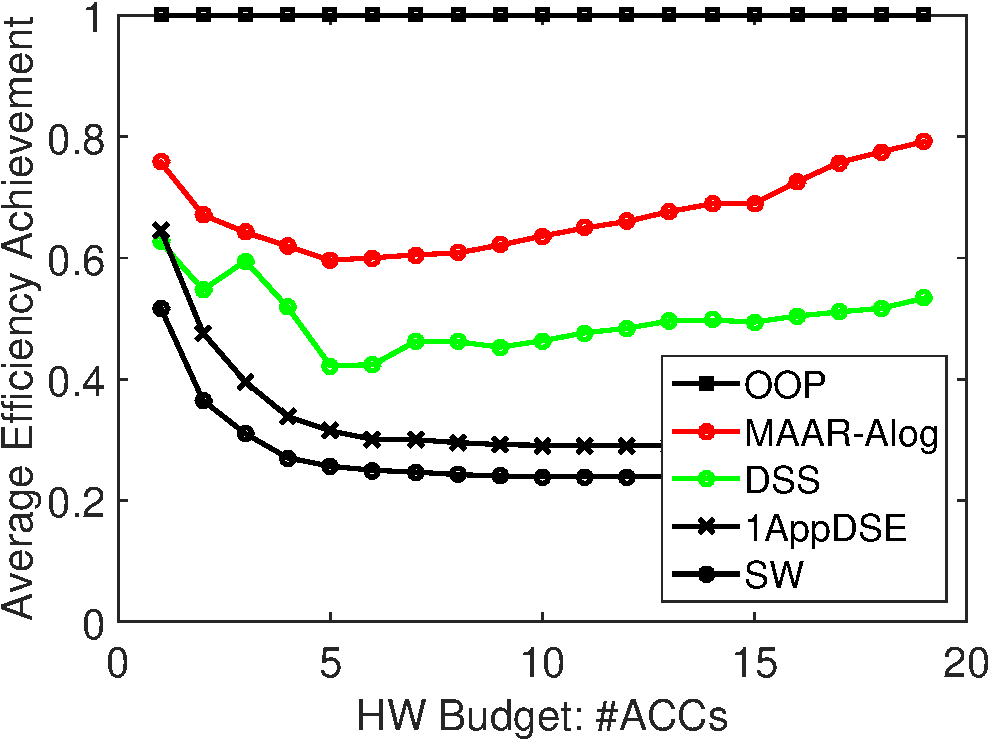
\includegraphics[width=.48\linewidth]{fig/alloop.pdf}\label{fig:alloop}}
		\hfill
		\subfloat[Cumulative Probability (ACCs=12)] {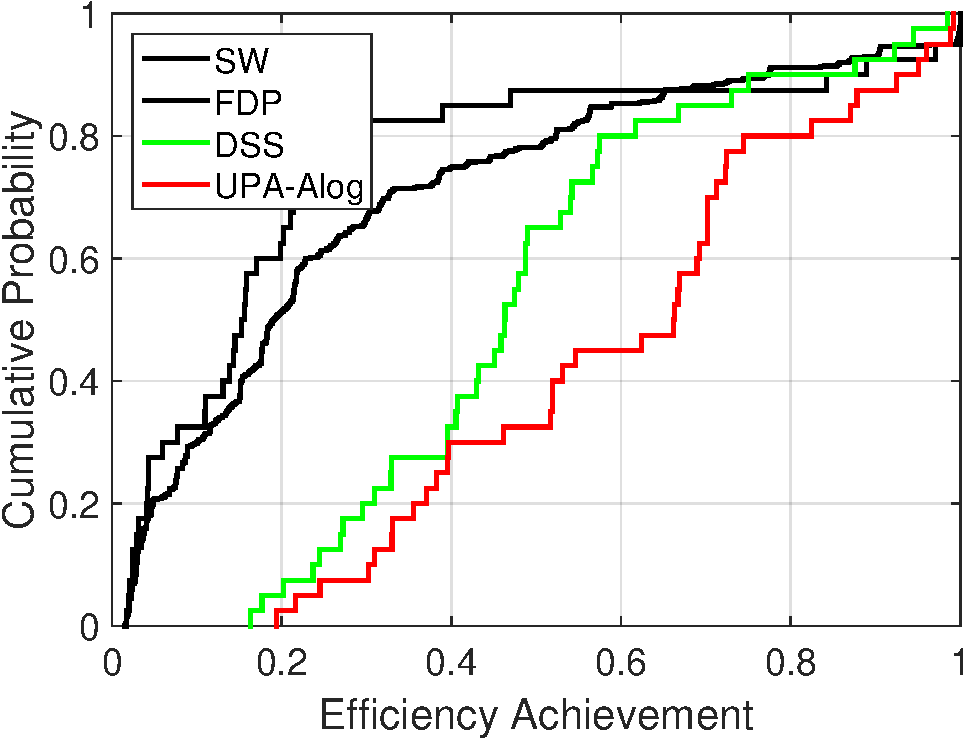
\includegraphics[width=.48\linewidth]{fig/MAARoop12all.pdf}\label{fig:oop12all}}
	\vspace{-8pt}
	\caption{Efficiency Achievement $rEFF_{OOP}$}
	\label{fig:overalloop}
\end{figure}

\figref{fig:alloop} shows the average efficiency achievement ($rEEF_{OOP}$) across all applications of different DSEs. 
\newtext{
OOP always achieves 100\% efficiency compared to itself (i.e. vertical line $x=1$ if drawn), and is the upper bound.}
SW has the lowest efficiency achievement, only reaching about 24\% after ACCs>9. 
\newtext{
MAAR DSE uses $Alog$ evaluation and produces a much better efficiency achievement than other DSEs.}
On average across the HW budgets, MAAR has 1.35 times the efficiency achievement of DSS, and 2.12 times the achievement of 1AppDSE.
\newtext{
\figref{fig:alloop} also shows that MAAR line is going down when ACCs<5, while it raises after ACCs>5.} It means that MAAR has a lower improvement speed than OOP when the HW budget is less than 5. However, after this point, MAAR improves faster than OOP. As OOP has already accelerated almost all computationally expensive kernels, there are less potential efficiency improvement for OOP.  

\newtext{
\figref{fig:oop12all} is the cumulative probability of efficiency achievement with 12 ACCs budget. Similar to \figref{fig:sw12all}, the line positioned more toward the bottom right has a better efficiency improvement, and MAAR has a significantly higher achievement than 1appDSE and DSS.
47.5\% ($1-0.525$ in y-axis) of applications obtain at least 60\% (in x-axis) efficiency of their dedicated OPT platform, while 1appDSE and DSS only has 12.5\% ($1-0.875$) and 10\% ($1-0.9$) of applications respectively achieving the same efficiency.
}

%Since efficiency achievement is relative to OOP, the plot of DSE can also describe the improvement speed between the DSE and OOP.
%MAAR is decreasing while ACCs<5, and increasing while ACCs>5. This 